%\documentclass[handout]{beamer}
\documentclass[10pt]{beamer}
\usetheme[
  outer/progressbar=foot,
  outer/numbering=none
]{metropolis}
\usepackage{amsmath, amssymb, amsthm, mathtools,media9}
\usepackage[export]{adjustbox}

\usepackage[default]{sourcesanspro}
\usepackage[utf8]{inputenc}
\usepackage[T1]{fontenc}
\metroset{titleformat=smallcaps}

\usepackage{tikz}
\usetikzlibrary{mindmap,shadows}
\usepackage{animate}
\usepackage[compatibility=false]{caption}

\usepackage{subcaption}
\usepackage{graphicx}
\usetikzlibrary{spy,calc,patterns,arrows,decorations.pathmorphing,backgrounds,positioning,fit,petri,mindmap,trees,intersections}
\usepackage{graphicx}
\usepackage{keystroke}
\usepackage{color}
\usepackage{multicol}
%\usepackage{multimedia}
\usepackage{enumerate}
\usepackage{multirow}
\usepackage{pgfplots,tikz,tcolorbox}
\usepackage{appendixnumberbeamer}



\pgfplotsset{compat=newest}
%\expandafter\def\expandafter\insertshorttitle\expandafter{%
 % \insertshorttitle\hfill\insertframenumber\,/\,\inserttotalframenumber}
%\usepackage{enumitem}


%\usepackage[T1]{fontenc}
\usepackage{color,hyperref}
\definecolor{darkblue}{rgb}{0.0,0.0,0.5}
%\hypersetup{colorlinks,breaklinks,
%            linkcolor=darkblue,urlcolor=darkblue,
%            anchorcolor=darkblue,citecolor=darkblue}
\usetikzlibrary{patterns}
\usetikzlibrary{decorations.pathmorphing,backgrounds,positioning,fit,petri,mindmap,trees}
\usepgflibrary{arrows,shapes.geometric}
\usepgflibrary{shapes.symbols}
%\hypersetup{colorlinks,breaklinks,linkcolor=darkblue,urlcolor=darkblue,anchorcolor=darkblue,citecolor=darkblue}
\usetikzlibrary{spy,calc,patterns,arrows,decorations.pathmorphing,backgrounds,positioning,fit,petri,mindmap,trees,intersections}
\usepackage{color}
\usepackage{multirow}
\usetikzlibrary{arrows,positioning} 
\tikzset{
    %Define standard arrow tip
    >=stealth',
    %Define style for boxes
    punkt/.style={
           rectangle,
           rounded corners,
           draw=black, very thick,
           text width=8.5em,
           minimum height=2em,
           text centered},
    % Define arrow style
    pil/.style={
           ->,
           thick,
           shorten <=2pt,
           shorten >=2pt,}
}

%\usepackage[hang]{footmisc}
%\setlength\footnotemargin{10pt}

\setbeamertemplate{caption}[numbered]
\usepgfplotslibrary{statistics}

\usetikzlibrary{fadings}
\tikzfading[name=fade out,
  inner color=transparent!0, outer color=transparent!100]

\setbeameroption{show notes}


\newcommand{\network}[1]{
\begin{figure}[h]
\centering
\begin{tikzpicture}[scale = 1,-,draw=black!50, node distance=\layersep]
    \tikzstyle{neuron}=[circle,fill=black!25,minimum size=17pt,inner sep=0pt];
    \tikzstyle{unit}=[neuron, fill=red!50];
    \tikzstyle{spike}=[neuron, fill=blue!50];
 \def \radius {2cm}
% \def \margin {8}
 \def \n {6}
 \foreach \s in {1,...,\n}
  \node[unit] (\s) at ({360/\n * (\s - 1) - 180}:\radius) {$\s$};
 \foreach \s in {1,...,\n}
  \foreach \t in {\s,...,\n}
   \draw (\t) -- (\s);
 \foreach \s in {1,...,\n}
   \draw[very thick] (#1) -- (\s);
   \node[spike] (#1) at ({360/\n * (#1 - 1) - 180}:\radius) {};
\end{tikzpicture}
\end{figure}

}


\newcommand{\networkwc}[6]{
\begin{figure}[h]
\centering
\begin{tikzpicture}[scale = 1,-,draw=black!50, node distance=\layersep]
    \tikzstyle{neuron}=[circle,fill=black!25,minimum size=17pt,inner sep=0pt];
    \tikzstyle{unit}=[neuron, fill=red!50];
    \tikzstyle{spike}=[neuron, fill=blue!50];
 \def \radius {2cm}
% \def \margin {8}
 \def \n {6}
% \foreach \s in {1,...,\n}
  \node[unit] (1) at (- 180:\radius) {{\color{white}#1}};
   \node[unit] (2) at (- 120:\radius) {{\color{white}#2}};
     \node[unit] (3) at (- 60:\radius) {{\color{white}#3}};
   \node[unit] (4) at (0:\radius) {{\color{white}#4}};
  \node[unit] (5) at (60:\radius) {{\color{white}#5}};
   \node[unit] (6) at (120:\radius) {{\color{white}#6}};
 \foreach \s in {1,...,\n}
  \foreach \t in {\s,...,\n}
   \draw (\t) -- (\s);
% \foreach \s in {1,...,\n}
%   \draw[very thick] (#1) -- (\s);
%   \node[spike] (#1) at ({360/\n * (#1 - 1) - 180}:\radius) {};
\end{tikzpicture}
\end{figure}
}

\newcommand{\networkwcww}[6]{
\begin{figure}[h]
\centering
\begin{tikzpicture}[scale = 1,-,draw=black!50, node distance=\layersep]
    \tikzstyle{neuron}=[circle,fill=black!25,minimum size=17pt,inner sep=0pt];
    \tikzstyle{unit}=[neuron, fill=red!50];
    \tikzstyle{spike}=[neuron, fill=blue!50];
 \def \radius {2cm}
% \def \margin {8}
 \def \n {6}
% \foreach \s in {1,...,\n}
  \node[unit] (1) at (- 180:\radius) {{\color{white}#1}};
   \node[unit] (2) at (- 120:\radius) {{\color{white}#2}};
     \node[unit] (3) at (- 60:\radius) {{\color{white}#3}};
   \node[unit] (4) at (0:\radius) {{\color{white}#4}};
  \node[unit] (5) at (60:\radius) {{\color{white}#5}};
   \node[unit] (6) at (120:\radius) {{\color{white}#6}};
 \draw (1) edge node[below left] {\small $-1$} (2);
 \draw (2) edge node[below] {\small $-3$} (3);
  \draw (3) edge node[below right] {\small $-1$} (4);
   \draw (4) edge node[above right] {\small $3$} (5);
    \draw (5) edge node[above] {\small $-2$} (6);
         \draw (6) edge node[above left] {\small $3$} (1);
     \draw (2) edge node[right] {\small $2$} (6);
      \draw (3) edge node[left] {\small $3$} (5);
%  \draw (i) edge node[right] {\small $W_{ij} = W_{ji}$} (j);

 % \foreach \s in {1,...,\n}
%   \draw[very thick] (#1) -- (\s);
%   \node[spike] (#1) at ({360/\n * (#1 - 1) - 180}:\radius) {};
\end{tikzpicture}
\end{figure}
}

\newcommand{\mpm}[6]{
\begin{figure}[h]
\centering
\begin{tikzpicture}[scale = 1,-,draw=black!50, node distance=\layersep,>=stealth]
    \tikzstyle{neuron}=[circle,fill=black!25,minimum size=17pt,inner sep=0pt];
    \tikzstyle{unit}=[neuron, fill=red!50,thick];
 \def \radius {2cm}
% \def \margin {8}
 \def \n {6}
 \foreach \s in {1,...,\n}{
  \node[unit] (\s) at ({360/\n * (\s - 1) - 180}:\radius) {};
%  \node (S-\s) at ($(\s) + {360/\n * (\s - 1) - 180}:5mm$) {$s_i$};
}  

   \DoubleLine{1}{2}{<-,draw=black!50}{}{->,draw=black!50}{};
   \DoubleLine{1}{3}{<-,draw=black!50}{}{->,draw=black!50}{};
   \DoubleLine{1}{4}{<-,draw=black!50}{}{->,draw=black!50}{};
   \DoubleLine{1}{5}{<-,draw=black!50}{}{->,draw=black!50}{};
   \DoubleLine{1}{6}{<-,draw=black!50}{}{->,draw=black!50}{};
    \DoubleLine{2}{3}{<-,draw=black!50}{}{->,draw=black!50}{};
   \DoubleLine{2}{4}{<-,draw=black!50}{}{->,draw=black!50}{};
   \DoubleLine{2}{5}{<-,draw=black!50}{}{->,draw=black!50}{};
   \DoubleLine{2}{6}{<-,draw=black!50}{}{->,draw=black!50}{};
   \DoubleLine{3}{4}{<-,draw=black!50}{}{->,draw=black!50}{};
   \DoubleLine{3}{5}{<-,draw=black!50}{}{->,draw=black!50}{};
   \DoubleLine{3}{6}{<-,draw=black!50}{}{->,draw=black!50}{};
    \DoubleLine{4}{5}{<-,draw=black!50}{}{->,draw=black!50}{};
   \DoubleLine{4}{6}{<-,draw=black!50}{}{->,draw=black!50}{};
   \DoubleLine{5}{6}{<-,draw=black!50}{}{->,draw=black!50}{};

   \node[unit] (1) at (- 180:\radius) {{\color{white}#1}};
   \node[unit] (2) at (- 120:\radius) {{\color{white}#2}};
     \node[unit] (3) at (- 60:\radius) {{\color{white}#3}};
   \node[unit] (4) at (0:\radius) {{\color{white}#4}};
  \node[unit] (5) at (60:\radius) {{\color{white}#5}};
   \node[unit] (6) at (120:\radius) {{\color{white}#6}};
%   \draw[color=None] (i) edge node[right] {\small $W_{ij}$} (j);
%   \draw[color=None] (i) edge node[left] {\small $W_{ij}$} (j);
\end{tikzpicture}
\end{figure}

}

\newcommand\DoubleLine[7][1pt]{%
    \path(#2)--(#3)coordinate[at start](h1)coordinate[at end](h2);
    \draw[#4]($(h1)!#1!90:(h2)$)-- node [left=-.75mm] {#5} ($(h2)!#1!-90:(h1)$); 
    \draw[#6]($(h1)!#1!-90:(h2)$)-- node [right=-.75mm] {#7} ($(h2)!#1!90:(h1)$);
    }


\title{Simulating RNNs on GPUs}
\subtitle{Working Title}
%\institute{SUTD}
\author{Zhangsheng Lai}
%\date{\today}

\newcommand{\sol}{\textbf{Solution\\}}
\pgfmathdeclarefunction{gauss}{2}{%
  \pgfmathparse{1/(#2*sqrt(2*pi))*exp(-((x-#1)^2)/(2*#2^2))}%
}
%\pgfmathdeclarefunction{gauss1}{2}{%
  %\pgfmathparse{(1/(#2*sqrt(2*pi))*exp(-((-x-#1)^2)/(2*#2^2)))*exp(-x)}%
%}
\pgfmathdeclarefunction{gauss2}{2}{%
  \pgfmathparse{(1/(#2*sqrt(2*pi))*exp(-0.5*abs(x)-#1)*(sqrt(abs(x)))}%
}

%\pgfmathdeclarefunction{gauss2}{2}{%
  %\pgfmathparse{(1/(#2*sqrt(2*pi))*exp(-((x-#1)^2)/(2*#2^2)))*exp(x)}%
%}
\pgfmathdeclarefunction{gauss1}{2}{%
  \pgfmathparse{(1/(#2*sqrt(2*pi))*exp(-0.5*x-#1)*(sqrt(x))}%
}
\def\checkmark{\tikz\fill[scale=0.4](0,.35) -- (.25,0) -- (1,.7) -- (.25,.15) -- cycle;}

\newcommand*{\Perm}[2]{{}^{#1}\!P_{#2}}%
\newcommand*{\Comb}[2]{{}^{#1}C_{#2}}%
\begin{document}


\begin{frame}
\titlepage
\end{frame}


%\begin{frame}
%\tableofcontents
%\end{frame}



\begin{frame}{Mult-layer Perceptron}
\begin{figure}[h]
\centering

\def\layersep{2.5cm}

\begin{tikzpicture}[scale = 1,shorten >=1pt,->,draw=black!50, node distance=\layersep]
    \tikzstyle{every pin edge}=[<-,shorten <=1pt]
    \tikzstyle{neuron}=[circle,fill=black!25,minimum size=17pt,inner sep=0pt]
    \tikzstyle{input neuron}=[neuron, fill=green!50];
    \tikzstyle{output neuron}=[neuron, fill=red!50];
    \tikzstyle{hidden neuron}=[neuron, fill=blue!50];
    \tikzstyle{annot} = [text width=4em, text centered]

    % Draw the input layer nodes
    \foreach \name / \y in {1,...,3}
    % This is the same as writing \foreach \name / \y in {1/1,2/2,3/3,4/4}
        %\node[input neuron, pin=left:Input \#\y] (I-\name) at (0,-\y) {$x_\y$};
	\node[input neuron] (I-\name) at (0,-\y) {$x_\y$};
		\node[input neuron] (I-4) at (0,-4) {\small $+1$};

    % Draw the hidden layer nodes
    \foreach \name / \y in {1,...,5}
        \path[yshift=0.5cm]
            node[hidden neuron] (H-\name) at (\layersep,-\y cm) {};
  \path[yshift=0.5cm]
            node[hidden neuron] (H-5) at (\layersep,-5 cm) {\small $+1$};
    % Draw the output layer node
    \node[output neuron,pin={[pin edge={->}]right:$h_{W,b}(x) = f(z_{1}^{(3)}) = a_{1}^{(3)}$}, right of=H-3] (O) {};

    % Connect every node in the input layer with every node in the
    % hidden layer.
    \foreach \source in {1,...,4}
        \foreach \dest in {1,...,4}
            \path (I-\source) edge (H-\dest);

    % Connect every node in the hidden layer with the output layer
    \foreach \source in {1,...,5}
        \draw (H-\source)  edge node[above] {\small $a^{(2)}_{\source}$}(O);

    % Annotate the layers
    \node[annot,above of=H-1, node distance=1cm] (hl) {Hidden layer};
    \node[annot,left of=hl] {Input layer};
    \node[annot,right of=hl] {Output layer};
\end{tikzpicture}
\caption{Multi-layer perceptron}
\label{fig:neural network}
\end{figure}
\end{frame}

\begin{frame}{}
\section{Hopfield Networks and Boltzmann Machines}
\end{frame}



\begin{frame}{Hopfield Networks}
\networkwc{1}{-1}{1}{1}{-1}{1}
\end{frame}

\begin{frame}{Hopfield Networks}
\networkwc{1}{0}{1}{1}{0}{1}
\end{frame}

\begin{frame}{Hopfield Networks}
\begin{figure}[h]
\centering
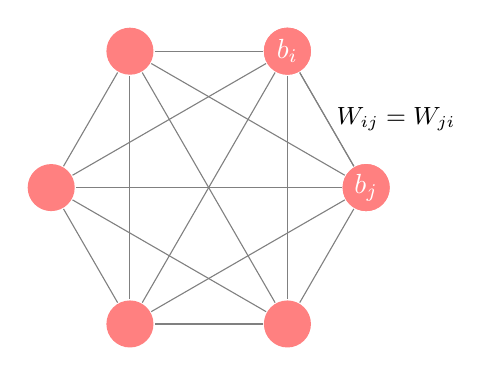
\begin{tikzpicture}[scale = 1,-,draw=black!50, node distance=\layersep]
    \tikzstyle{neuron}=[circle,fill=black!25,minimum size=17pt,inner sep=0pt];
    \tikzstyle{unit}=[neuron, fill=red!50,thick];
 \def \radius {2cm}
% \def \margin {8}
 \def \n {6}
 \foreach \s in {1,...,\n}{
  \node[unit] (\s) at ({360/\n * (\s - 1) - 180}:\radius) {};
%  \node (S-\s) at ($(\s) + {360/\n * (\s - 1) - 180}:5mm$) {$s_i$};
}  
 \foreach \s in {1,...,\n}
  \foreach \t in {\s,...,\n}
   \draw (\t) -- (\s);
   \node[unit](i) at ({60 }:\radius) {{\color{white}$b_i$}};
   \node[unit](j) at ({360}:\radius) {{\color{white}$b_j$}};
   \draw (i) edge node[right] {\small $W_{ij} = W_{ji}$} (j);

   \end{tikzpicture}
\end{figure}
\begin{align*}
\text{Energy configuration, }E &= -\sum_{i<j}W_{ij}x_ix_j - \sum_ib_i x_i \\
\text{Energy gap, } \Delta E_i &= E(x_i = 0) - E(x_i = 1) = \sum_jW_{ij}x_j +b_i\\
\text{Update rule, }x_i:&=\begin{cases}
+1 & \sum_jW_{ij}x_j +b_i \geq 0\\
-1 & \text{otherwise}
\end{cases}
\end{align*}
\end{frame}

\note{\scriptsize
\begin{itemize}
\item composed of primitive computing elements called units
\item units has two states, on or off, represented by $\{1,-1\}$ or $\{1,0\}$
\item connected to each other by bi-directional links
\item adopts these states as a function of the states of its neighbouring units and weights of its links to them, it is a probabilistic function for a Boltzmann machine.
\item weights can take on any real value
\item a unit being on or off is taken to mean that the system currently accepts or rejects some elemental hypothesis of the domain
\item weight on a link represents a weak pairwise constrain between two hypothesis
\item positive (negative) weights indicate that two hypothesis support (contradict) one another with other things being equal
\item link weights are symmetric, having the same strength in both directions
\end{itemize}
}


\begin{frame}{Hopfield Networks}
\networkwcww{1}{0}{0}{0}{0}{1}
\end{frame}

\begin{frame}{Hopfield Networks}
\networkwcww{1}{1}{0}{0}{0}{1}
\end{frame}

\begin{frame}{Hopfield Networks}
\networkwcww{0}{0}{1}{1}{1}{0}
\end{frame}

\note{
\scriptsize
\begin{itemize}
\item Updating of Hopfield networks is done 	sequentially usually in a randomized order. Parallel updating might increase the energy instead.
%Asynchronous: one unit is updated at a time, can be done randomly or in a pre-defined order. Synchronous: all units are updated at the same time.
\item Hopfield networks always make decisions to reduce the energy and makes it impossible to escape from local minima.
\item random noise can help us escape from poor minima, by starting with lots of noise so its easy to cross energy barriers and gradually decrease the noise so the system ends in a deep minimum. This is called simulated annealing.
\end{itemize}
}


\begin{frame}{Boltzmann Machines}
\begin{figure}[h]
\centering
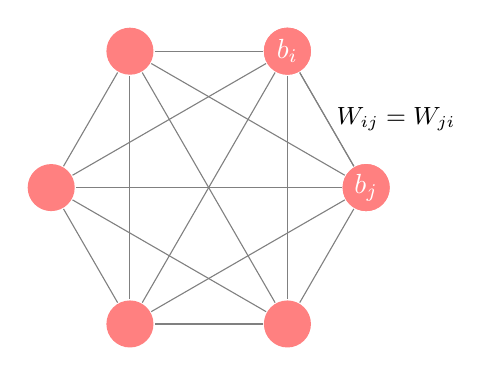
\begin{tikzpicture}[scale = 1,-,draw=black!50, node distance=\layersep]
    \tikzstyle{neuron}=[circle,fill=black!25,minimum size=17pt,inner sep=0pt];
    \tikzstyle{unit}=[neuron, fill=red!50,thick];
 \def \radius {2cm}
% \def \margin {8}
 \def \n {6}
 \foreach \s in {1,...,\n}{
  \node[unit] (\s) at ({360/\n * (\s - 1) - 180}:\radius) {};
%  \node (S-\s) at ($(\s) + {360/\n * (\s - 1) - 180}:5mm$) {$s_i$};
}  
 \foreach \s in {1,...,\n}
  \foreach \t in {\s,...,\n}
   \draw (\t) -- (\s);
   \node[unit](i) at ({60 }:\radius) {{\color{white}$b_i$}};
   \node[unit](j) at ({360}:\radius) {{\color{white}$b_j$}};
   \draw (i) edge node[right] {\small $W_{ij} = W_{ji}$} (j);

   \end{tikzpicture}
\end{figure}
\begin{align*}
E &= -\sum_{i<j}W_{ij}x_ix_j - \sum_ib_i x_i \\
\Delta E_i &= E(x_i = 0) - E(x_i = 1) = \sum_jW_{ij}x_j +b_i\\
&\mathbb{P}(x_i=1) = \frac{1}{1+e^{-\Delta E_i/\tau}}
\end{align*}
\end{frame}

\note{
\scriptsize
\begin{itemize}

\item replace the binary threshold units by binary stochastic units that make biased random decisions
\item temperature variable controls the amount of noise 
\item when $\tau \to 0$ we get back the Hopfield network
\item for $\tau_1 > \tau_2$, we are less likely to go to a lower energy state compared to in $\tau_1$ compared to $\tau_2$, i.e. more likely to go to a higher energy state when the temperature is higher. This allows us to escape from local minimum and arrive at the global minimum.
\end{itemize}
}



\begin{frame}{Boltzmann Machines}
%\begin{align*}
%\mathbb{P}(x_i=1) = \frac{1}{1+e^{-\Delta E_i/\tau}}
%\end{align*}
\begin{figure}[h]
\centering
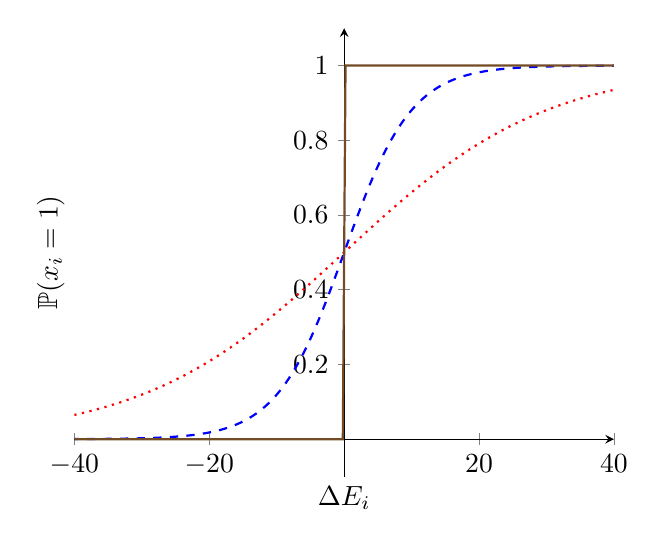
\begin{tikzpicture}
    \begin{axis}[
        domain=-80:80,
        xmin=-40, xmax=40,
        ymin=-0.1, ymax=1.1,
        samples=400,
        axis y line=center,
        axis x line=middle,
        >=stealth,
        x label style={at={(axis description cs:0.5,0)},anchor=north},
    y label style={at={(axis description cs:0,.5)},rotate=90,anchor=south},
        xlabel = $\Delta E_i$,
        ylabel = {$\mathbb{P}(x_i=1)$}
    ]
        \addplot+[mark=none,thick,dashed,color=blue] {1/(1+e^(-x/5))};
        \addplot+[mark=none,thick,dotted] {1/(1+e^(-x/15))};
        \addplot+[mark=none,thick] {1/(1+e^(-x/0.01))};
    \end{axis}
\end{tikzpicture}
\caption{$\tau=0$ (solid), $\tau=5$ (dashed), $\tau=15$ (dotted)}
\end{figure}
\end{frame}


\begin{frame}{}
\section{McCulloh-Pitts Machines}
\end{frame}

\begin{frame}{McCulloh-Pitts Machines}
\mpm{1}{0}{1}{0}{0}{1}

\end{frame}


\begin{frame}{McCulloh-Pitts Machines}
\begin{figure}[h]
\centering
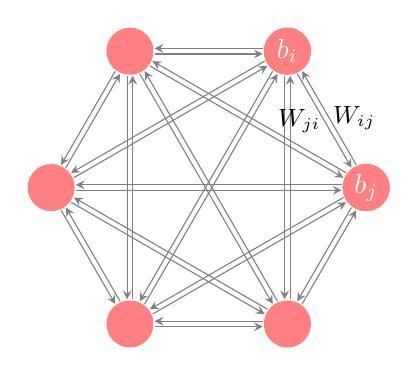
\begin{tikzpicture}[scale = 1,-,draw=black!50, node distance=\layersep,>=stealth]
    \tikzstyle{neuron}=[circle,fill=black!25,minimum size=17pt,inner sep=0pt];
    \tikzstyle{unit}=[neuron, fill=red!50,thick,];
 \def \radius {2cm}
% \def \margin {8}
 \def \n {6}
 \foreach \s in {1,...,\n}{
  \node[unit] (\s) at ({360/\n * (\s - 1) - 180}:\radius) {};
%  \node (S-\s) at ($(\s) + {360/\n * (\s - 1) - 180}:5mm$) {$s_i$};
}  

   \DoubleLine{1}{2}{<-,draw=black!50}{}{->,draw=black!50}{};
   \DoubleLine{1}{3}{<-,draw=black!50}{}{->,draw=black!50}{};
   \DoubleLine{1}{4}{<-,draw=black!50}{}{->,draw=black!50}{};
   \DoubleLine{1}{5}{<-,draw=black!50}{}{->,draw=black!50}{};
   \DoubleLine{1}{6}{<-,draw=black!50}{}{->,draw=black!50}{};
    \DoubleLine{2}{3}{<-,draw=black!50}{}{->,draw=black!50}{};
   \DoubleLine{2}{4}{<-,draw=black!50}{}{->,draw=black!50}{};
   \DoubleLine{2}{5}{<-,draw=black!50}{}{->,draw=black!50}{};
   \DoubleLine{2}{6}{<-,draw=black!50}{}{->,draw=black!50}{};
   \DoubleLine{3}{4}{<-,draw=black!50}{}{->,draw=black!50}{};
   \DoubleLine{3}{5}{<-,draw=black!50}{}{->,draw=black!50}{};
   \DoubleLine{3}{6}{<-,draw=black!50}{}{->,draw=black!50}{};
    \DoubleLine{4}{5}{<-,draw=black!50}{\small$W_{ji}$}{->,draw=black!50}{\small$W_{ij}$};
   \DoubleLine{4}{6}{<-,draw=black!50}{}{->,draw=black!50}{};
   \DoubleLine{5}{6}{<-,draw=black!50}{}{->,draw=black!50}{};

   \node[unit](i) at ({60 }:\radius) {{\color{white}$b_i$}};
   \node[unit](j) at ({360}:\radius) {{\color{white}$b_j$}};
%   \draw[color=None] (i) edge node[right] {\small $W_{ij}$} (j);
%   \draw[color=None] (i) edge node[left] {\small $W_{ij}$} (j);
\end{tikzpicture}
\end{figure}
\begin{align*}
E(y,x|\theta) &= -\sum_{ji \in E}W_{ji}y_jx_i- \sum_{j \in V}b_j s_j- \sum_{i \in V}b_i s_i\\
\Gamma_{yx} &=\exp\left(-\frac{1}{2\tau}E(y,x|\theta)+\frac{1}{2\tau}E(x,x|\theta)\right)\\
\end{align*}
where $G=(V,E)$ digraph, $\theta = (W, b, \tau)$
\end{frame}

\begin{frame}{McCulloh-Pitts Machines}

\begin{align*}
E(y,x|\theta) &= -\sum_{ji \in E}W_{ji}y_jx_i- \sum_{j \in V}b_j s_j- \sum_{i \in V}b_i s_i\\
\Gamma_{yx} &=\exp\left(-\frac{1}{2\tau}E(y,x|\theta)+\frac{1}{2\tau}E(x,x|\theta)\right):=\lambda_j = \exp\left(\frac{1}{2\tau}s_jz_j\right)\\
\end{align*}
$s_j = 1 - 2x_j$ and $z_j = \sum_{ji \in E}W_{ji}x_i + b_j$
\end{frame}

\begin{frame}{McCulloh-Pitts Machines}

\begin{align*}
E(x^{(n+1)},x^{(n)}|\theta) &= -\sum_{ji \in E}W_{ji}x^{(n+1)}_jx^{(n)}_i- \sum_{j \in V}b_j s_j- \sum_{i \in V}b_i s_i\\
\Gamma_{x^{(n+1)}x^{(n)}} &=\exp\left(-\frac{1}{2\tau}E(x^{(n+1)},x^{(n)}|\theta)+\frac{1}{2\tau}E(x^{(n)},x^{(n)}|\theta)\right)\\
\end{align*}
\end{frame}

\begin{frame}{McCulloh-Pitts Machines}

\end{frame}



\begin{frame}{Introduction}
\emph{Homotopy type theory} is a new branch of mathematics that combines \emph{homotopy theory} and \emph{type theory}. 
\begin{itemize}
\item \textbf{Homotopy theory:} an outgrowth of algebraic topology and homological algebra, with relationship with higher category.
\item \textbf{Type theory:} branch of mathematical logic and theoretical computer science.
\end{itemize}
\end{frame}


\begin{frame}{Introduction}
\begin{alertblock}{Russell's Paradox}
Let $R$ be the set of sets that are not members of themselves. If $R$ is not a member of itself, then it must contain itself, and if it contains itself, it then contradicts its own definition as the set of all sets that are not members of themselves. This contradiction is Russell's paradox.
\begin{align*}
R = \{x ~|~ x \notin x\}  \text{, then, } R \in R \Leftrightarrow R \notin R
\end{align*}
\end{alertblock}
\end{frame}


\begin{frame}{Introduction}
\begin{figure}[h]
\centering
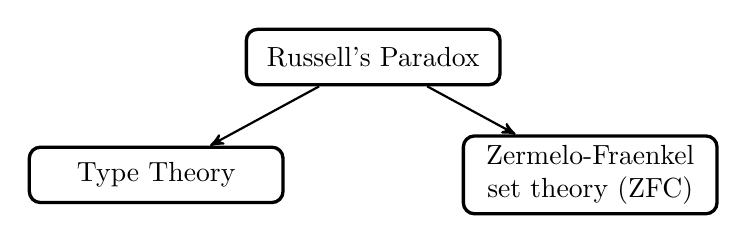
\begin{tikzpicture}[node distance=1cm, auto,]
 %nodes
 \node[punkt] (t) {Russell's Paradox};
 \node[below=of t] (dummy) {};
 \node[punkt,right=of dummy](o) { Zermelo-Fraenkel set theory (ZFC)};
 \draw[->,thick] (t) -- (o);
 
 \node[punkt,left=of dummy] (d) {Type Theory};
  \draw[->,thick] (t) -- (d);

\end{tikzpicture}
\caption{Ways to avoid Russell's Paradox}
\end{figure}
\note{
\begin{itemize}
\item the set of all airplanes are not members of themselves, but the set of all non-airplanes, are members of themselves.
\item The essential difference between Russell's and Zermelo's solution to the paradox is that Zermelo altered the axioms of set theory while preserving the logical language in which they are expressed (the language of ZFC, with the help of Skolem, turned out to be first-order logic) while Russell altered the logical language itself.
\end{itemize}
}
\end{frame}

\begin{frame}{Introduction}
Analysing the paradox, the problem stems from the set theory's liberal formation principles of allowing inhomogeneous sets. More specifically, a collection of objects in a set may contain members which can only be defined by means of the collection as a whole.

\begin{exampleblock}{Example}
Consider the collection of propositions, which supposed to contain a proposition stating that ``all propositions are either true or false''. The analysis we made earlier suggests that this proposition would not be legitimate unless ``all propositions'' referred to some already definite collection.
\end{exampleblock}


\end{frame}

\begin{frame}{Introduction}
Over the years, type theory was further developed by many other people. The type theory that we consider in HoTT is \emph{Martin L$\ddot{\text{o}}$f type theory}, which has applications in computer science and the theory of programming languages. 

The clear reasoning principles associated with the construction of types also form the basis of modern \emph{computer proof assistants}, with \href{https://coq.inria.fr/}{Coq} and \href{http://wiki.portal.chalmers.se/agda/pmwiki.php}{Agda} being some of the more popular ones.

\note{
\begin{itemize}
\item In short, we could see it as some sort of self referencing; an element of the set is referencing to the set it is contained in and this is not good!
\item The \emph{type} in \emph{type theory} is similar to the data-types we have in programming languages.
\end{itemize}
}
\end{frame}

\begin{frame}{Homotopy Theory}
A \emph{homotopy} between a pair of continuous mappings $f: X \to Y$ and $g: X \to Y$ is a continuous map
\begin{align*}
H: X \times [0,1] \to Y
\end{align*}
satisfying $H(x,0) = f(x)$ and $H(x,1) = g(x)$, i.e. some form of ``continuous deformation'' of $f$ into $g$.
\end{frame}


%\begin{frame}{Homotopy Theory}
%\begin{block}{Homotopy Interpretation}
%Here we will rewrite $a=_Ab$ as $\text{Id}_A(a,b)$
%\begin{align*}
%a, b &:A \\
%p, q &: \text{Id}_A(a,b)\\
%\alpha, \beta &: \text{Id}_{\text{Id}_A(a,b)}(p,q)\\
%\ldots &: \text{Id}_{\text{Id}_{\text{Id}\ldots}}\ldots
%\end{align*}
%\end{block}
%\end{frame}


\begin{frame}{Type Theory}
The basic concept of type theory is that we have \emph{terms} and \emph{types} as compared to elements and sets in set theory. The term $a$ that is of type $A$ is written as
\begin{align*}
a :A
\end{align*} 
we can also say that $a$ is an inhabitant of $A$.


%Type theory also has this very important conception of \emph{proposition as types} which is how it is used to formalize mathematics and verify the correctness of proofs.
\note{There is an inclination to just pass it off as just a change in notation from $\in$ to :, but there is more than this to it. }
\end{frame}

\begin{frame}{Type Theory}
There are two ways of interpreting a type:
\begin{itemize}
\item when $A$ is used to represent a proposition, then the $a$ in $a:A$ may be seen as a witness to the provability of $A$ or evidence to the truth of $A$. This important concept of \emph{proposition as types} is how it is used to formalize mathematics and verify the correctness of proofs.
\item the type $A$ can also be treated more like a set than a proposition, then ``$a : A$'' is analogous to ``$a \in A$'' but they differ in the the former is a \emph{judgment} whereas the latter is \emph{proposition}. 
\end{itemize}
\end{frame}

\begin{frame}{Type Theory}
\begin{exampleblock}{Example}
Here we have a proposition ``$A$ is isomorphic to $B$'' stated in type theory notation:
\begin{align*}
\text{Iso($A,B$)}:\equiv \sum_{f:A\to B}\sum_{g:B\to A}\left(\left(\prod_{x:A}g(f(x))=x\right)\times \left(\prod_{y:B}f(g(y))=y\right)\right)
\end{align*}
and to be able to find a term $p:\text{Iso}(A,B)$ is same as constructing an isomorphism between $A$ and $B$. Proofs are treated as mathematics objects like functions, groups and permutations.
\end{exampleblock}
\end{frame}

\begin{frame}{Type Theory}
\begin{exampleblock}{Example}
There exists two irrational numbers such that its sum is rational.
\begin{align*}
 \exists~ x, y \in \mathbb{R}\setminus\mathbb{Q} \text{  such that  } x + y \in \mathbb{Q}
\end{align*}
\end{exampleblock}
%If you look at the portions with $\in$, they look symbolically the same but they have different semantics. The $x, y \in \mathbb{R}$ is asserting that $x, y$ are `really' in $\mathbb{R}$, but $x+y\in \mathbb{Q}$ is a proposition\footnote{A proposition is a statement which has truth value: it is either true or false.}, it is `suggesting' that $x+y$ can be rational, but unless we can find an example(evidence), we cannot claim that $x+y \in \mathbb{Q}$.
\end{frame}

\begin{frame}{Type Theory}
\begin{block}{Comparison with Set Theory}
\begin{table}[h]
\centering
\small
\begin{tabular}{p{5cm}|p{5cm}}
\hline
Set Theory & Type Theory \\
\hline
 ``membership'' is a relation that may or may not hold between an element $a$ and a set $A$ & every term belongs to some type; A type needs to be formed first before introduction rules are used to construct the terms of the type.\\
 \hline
$\mathbb{N}$ in set theory: & $\mathbb{N}$ in type theory:\\$\{\varnothing, \{\varnothing\}, \{\varnothing, \{\varnothing\}\}, \ldots\}$&$0: \mathbb{N}$ and succ: $\mathbb{N} \to \mathbb{N}$\\
 \{$0, 1, 2, \ldots\}$ & $1:\equiv \text{succ}(0), 2:\equiv \text{succ}(1), \ldots$\\ 
 
\end{tabular}
\end{table}

%\begin{itemize}
%\item in set theory, ``membership'' is a relation that may or may not hold between an element $a$ and a set $A$
%\end{itemize}
\end{block}
\end{frame}


\begin{frame}{Type Theory}
\begin{block}{Equalities}
\emph{Judgmental equality} or \emph{Definitional equality} is equality of the syntax 	and is denote by $:\equiv$. \\For example,
\begin{align*}
(x+1)^2  :\equiv x^2+2x+1
\end{align*}
since it is easily obtained by algebraic expansion. \note{From the HoTT book, it says that it is helpful to think of this meaning "equality by definition" which is really exactly what it says.}

\emph{Propositional equality} on the other hand is though of as a type\footnote{since equality is a proposition and proposition are types}. For terms $a, b : A$, we have the type ``$a =_Ab$''. Only when $a =_Ab$ is inhabited can we say that $a$ and $b$ are (propositionally) equal, and this inhabitation comes in the form of a term for the type $a =_Ab$, i.e. $p:a =_Ab$ and $p$ should be viewed as evidence for the equality to hold.
\end{block}
\end{frame}


\begin{frame}{Type Theory}
\begin{block}{Function Types}
Let $A$ and $B$ be some types, then the type $A \to B$ is formed with domain $A$ and codomain $B$. For $f:A \to B$, giving it $a:A$ will produce an inhabitant of $B$, denoted $f(a)$.


The terms of this type is constructed by direct definition or $\lambda-$abstraction. Direct definition means we simply define $f :A \to B$ by giving an equation
\begin{align}
f(x): \equiv \Phi \label{eqn:directdefn}
\end{align}
where $\Phi$ is an expression which may contain $x$. Formation using $\lambda-$abstraction allows us to skip the naming of the term by writing
\begin{align*}
\lambda x.\Phi: A \to B
\end{align*}
which is the same term in (\ref{eqn:directdefn}). For the construction to be valid, we need to verify that $\Phi:B$ given $x:A$.
\note{
\begin{itemize}
\item unlike set theory, functions are primitive concepts in type theory; we explain what functions types are by prescribing what we can do with functions, how to construct them and what equalities they induce.
\item in set theory, a function $f:A \to B$ are defined as a subset $f \subseteq A \times B$
\begin{itemize}
\item for all $a \in A$ there exist $b \in B$ such that $(a,b) \in f$
\item for all $a \in A$ and $b, b' \in B$, if $(a,b)\in f$ and $(a,b')\in f$, $b=b'$.	
\end{itemize}
\end{itemize}
}
\end{block}
\end{frame}

\begin{frame}{Type Theory}
We can do computation by using either the definition or $\lambda-$abstraction.
\begin{align*}
f(a) \equiv \Phi' \equiv (\lambda x.\Phi)(a)
\end{align*}
where $\Phi'$ is the expression $\Phi$ in which all the occurrences of $x$ have been replaced by $a$.

Lastly, for any $f:A \to B$ we can construct a $\lambda-$abstraction $\lambda x.f(x)$, we can consider it to be definitionally equal to $f$
\begin{align*}
f: \equiv (\lambda x.f(x))
\end{align*}
and this equality is the \emph{uniqueness principle of function types}, because it shows that $f$ is uniquely determined by its values.
\end{frame}

\begin{frame}{Type Theory}
\begin{exampleblock}{Example}
Let both $A, B$ be the type of natural numbers, $\mathbb{N}$. 

Direct definition means we simply define $f :\mathbb{N} \to \mathbb{N}$ by giving an equation
\begin{align}
f(x): \equiv x+x \label{eqn:directdefnexp}%\tag{1}
\end{align}
where $\Phi$ is an expression which may contain $x$. Formation using $\lambda-$abstraction allows us to skip the naming of the term by writing
\begin{align*}
\lambda x.x+x: \mathbb{N} \to \mathbb{N}
\end{align*}
which is the same term in (\ref{eqn:directdefnexp}). We can do computation by 
\begin{align*}
(\lambda x.x+x) (2) \equiv 2 + 2
\end{align*}

\end{exampleblock}
\end{frame}


\begin{frame}{Type Theory}
\begin{alertblock}{Type Forming Rules:}
\begin{enumerate}
\item \textbf{Formation.} Tells us how to form new types.
\item \textbf{Introduction.} Also known as a \emph{constructor}, which specifies how to construct terms of a newly formed type.
\item \textbf{Elimination.} How to use the terms of that type.
\item \textbf{Computation.} Expresses how an eliminator acts on a constructor.
\item \textbf{Uniqueness Principle.} Expresses the uniqueness of maps into or out of that type.
\end{enumerate}
\end{alertblock}

\end{frame}




\begin{frame}{Type Theory}
\begin{block}{Inference Rules}
\begin{align*}
\frac{\vdash X: Type\qquad \vdash A:Type}{\vdash (X \to A): Type}\tag{Type Formation}\\
\frac{x:X\vdash a(x):A}{\vdash (x \mapsto a(x)):X \to A} \tag{Type Introduction}\\
\frac{\vdash f:(X \to A) \qquad \vdash x:X}{x:X \vdash f(x):A}\tag{Type Elimination}\\
\frac{x:X\vdash a(x):A \qquad \vdash x:X}{\vdash (\lambda(x:X).a)(y)\equiv a[y\,/\, x]:A[y\,/\, x]}\tag{Type Computation}\\
\frac{\vdash f: (X \to A)}{\vdash f \equiv (\lambda x.f(x)):X \to A} \tag{Uniqueness}
\end{align*}
the $\vdash$ symbol is called the turnstile and for $x:A\vdash a(x):A$, it should be read as 
\begin{quote}
\small In the context of variable $x$ of type $X$, the expression $a(x)$ has type $A$.
\end{quote}
\end{block}
\end{frame}



\begin{frame}{Comparison of the Different Points of View}
\begin{table}[h]
\centering
\small
\begin{tabular}{llll}
\hline
Types & Logic & Sets & Homotopy\\
\hline
$A$ & proposition & set & space\\
$a: A$  &proof  &element  &point  \\  
$B(x)$    & predicate &family of sets  &fibration  \\
$b(x):B(x)$      &conditional proof  & family of elements &section  \\
\textbf{0,1} &$\bot, \top$  & $\varnothing,\{\varnothing\}$ &$\varnothing, \ast$  \\
 $A + B$    & $A \vee B$ & disjoint union & coproduct \\
$A \times B$    & $A \wedge B$ & set of pairs & product space \\
$A \to B$    & $A \implies B$ & set of functions & function space \\
$\sum_{x:A}B(x)$      & $\exists_{x:A}B(x)$ & disjoint sum & total space \\
$\prod_{x:A}B(x)$       & $\forall_{x:A}B(x)$ & product & space of sections \\
Id$_{A}$   & equality = & $\{(x,x)\mid x \in A\}$ &  path space of $A^I$\\
\hline
\end{tabular}
\caption{Comparing the points of view on type-theoretic operations.}
\end{table}
\end{frame}



\begin{comment}%%%%%%%%%%%%%%%%%%%%%%%%%%%%%%%%

\begin{frame}{Type Theory}
\begin{block}{Universe and Families}

\end{block}
\end{frame}


\begin{frame}{Type Theory}
\begin{block}{Dependent Function Types ($\Pi-$types)} 
Let $A, B: \mathcal{U}$ be any two types, we can introduce the type $A \times B$ which is the \emph{cartesian product} of type theory. We expect the terms of $A \times B$ to be of the form $(a,b)$ like what we are familiar with in set theory.
\end{block}
\end{frame}


\begin{frame}{Type Theory}
The basic concept of type theory is that we have \emph{terms}, \emph{types} and \emph{universe}. The term $a$ that is of type $A$ is written as
\begin{align*}
a :A
\end{align*} 
and universes denoted by $\mathcal{U}$ are simply types whose terms are also types
\begin{align*}
A : \mathcal{U}
\end{align*}
Type theory also has this very important conception of \emph{proposition as types} which is how it is used to formalize mathematics and verify the correctness of proofs.
\note{There is an inclination to just pass it off as just a change in notation from $\in$ to :, but there is more than this to it. }
\end{frame}


\begin{frame}{Type Theory}
\begin{block}{Natural Numbers}
Before we look at how natural numbers are constructed in type theory, we shall briefly visit the set-theoretic definition of natural numbers. Zermelo-Fraenkel set theory defines natural numbers recursively by 
\begin{alignat*}{2}
0 &= \varnothing & &\\
1 &= \{0\}& &=\{\varnothing\} \\
2 &= \{1\}& &=\{\{\varnothing\}\} \\
3 &= \{2\}& &=\{\{\{\varnothing\}\}\} \\
 &  &\vdots &
\end{alignat*}
\end{block}
\end{frame}

\begin{frame}{What is a type?}
\begin{exampleblock}{Example}
There exists two irrational numbers such that its sum is rational.
\begin{align*}
 \exists~ x, y \in \mathbb{R}\setminus\mathbb{Q} \text{  such that  } x + y \in \mathbb{Q}
\end{align*}
\end{exampleblock}
If you look at the portions with $\in$, they look symbolically the same but they have different semantics. The $x, y \in \mathbb{R}$ is asserting that $x, y$ are `really' in $\mathbb{R}$, but the $x+y\in \mathbb{Q}$ is a proposition\footnote{A proposition is a statement which has truth value: it is either true or false.}, it is `suggesting' that $x+y$ can be rational, but unless we can find an example(evidence), we cannot claim that $x+y \in \mathbb{Q}$.
\end{frame}

\begin{frame}{What is a type?}
Summing it up:\\
In type theory,  $n:\mathbb{N}$ is a judgment; it cannot change, but in set theory the $n \in \mathbb{N}$ is a proposition; it can be true or false.
\note{We shall now go on to another big difference between set and type theory, which is the notion of equality.}
\end{frame}


\begin{frame}{Equalities in Type Theory}

\textbf{Judgmental equality} is equality of the syntax 	and is denote by $:\equiv$. An example will be 
\begin{align*}
(x+1)^2 : \equiv x^2+2x+1
\end{align*}
since it is easily obtained by algebraic expansion. \note{From the HoTT book, it says that it is helpful to think of this meaning "equality by definition" which is really exactly what it says.}

\textbf{Propositional equality} on the other hand is though of as a type\footnote{since equality is a proposition and proposition are types}. For terms $a, b : A$, we have the type ``$a =_Ab$''. Only when $a =_Ab$ is inhabited can we say that $a$ and $b$ are (propositionally) equal, and this inhabitation comes in the form of a term for the type $a =_Ab$, i.e. $p:a =_Ab$ and $p$ should be viewed as evidence for the equality to hold.
\end{frame}


\begin{frame}{How to Specify a Type}
\begin{alertblock}{Rules:}
\begin{enumerate}
\item \textbf{Formation.} Tells us how to form new types.
\item \textbf{Introduction.} Also known as a \textbf{constructor}, which specifies how to construct terms of a newly formed type.
\item \textbf{Elimination.} How to use the terms of that type.
\item \textbf{Computation.} Expresses how an eliminator acts on a constructor.
\item \textbf{Uniqueness Principle.} Expresses the uniqueness of maps into or out of that type.
\end{enumerate}
\end{alertblock}
\end{frame}

\begin{frame}{Dependent function types ($\Pi$-types)}
\textbf{$\Pi$-types} or \textbf{dependent function type} are types where the elements are \emph{functions} whose codomain can vary depending on the element of the domain to which the function is applied. Given a type $A : \mathcal{U}$ and a family $B:A\to\mathcal{U}$ we write the constructed dependent functions as 
\begin{align*}
\prod_{(x:A)}B(x)
\end{align*}
\note{the codomain of the function depends on the term $a:A$.}
\end{frame}



\begin{frame}{Function Types}
For some types $A$ and $B$, we would now like to construct the type $A \to B$ of functions domain $A$ and codomain $B$. We can either construct elements of $A \to B$ by defining a function, $f : \mathbb{R} \to \mathbb{R}$ by 
\begin{align*}
f(x):\equiv x^2+1
\end{align*}
or by using $\lambda-$abstraction
\begin{align*}
\lambda (x:\mathbb{R}).x^2+1:\mathbb{R} \to \mathbb{R}
\end{align*}
Both constructions above give the same function, just that the latter does not introduce a name for the function.
\end{frame}

\begin{frame}{Function Types}
We can also construct a \textbf{constant function} 
\begin{align*}
\lambda x.y:A \to B
\end{align*}
The type of the variable is generally omitted as it is inferable and by convention, the ``scope'' of the variable binding ``$\lambda x$'' is the rest of the expression, unless delimited by parenthesis. For example, $\lambda x.x+x$ is parsed as $\lambda x. (x+x)$ and not $(\lambda x.x) +x$ which is in fact ill-typed.
\end{frame}

\begin{frame}{Function Types}

\end{frame}


\begin{frame}{Universe and Families}

\end{frame}

\begin{frame}{Dependent function types ($\Pi$-types)}

\end{frame}

\begin{frame}{Dependent pair types ($\Sigma$-types)}

\end{frame}

\begin{frame}{Homotopy Theory}

\end{frame}


\begin{frame}{Things about HoTT}
\begin{enumerate}
\scriptsize
\item In type theory, we should think of types as being formed by definitions that define them, rather than by the contents of the types (which is what we do in set theory).
\item Univalent foundations: In type theory, one can have a universe $\mathcal{U}$, the terms of which themselves are types $A:\mathcal{U}$. Those types that are terms of $\mathcal{U}$ are called \emph{small types}. Like any type, $\mathcal{U}$ has the identity type $Id_{\mathcal{U}}$ which expresses the identity relation between small types. Thinks of types as spaces, $\mathcal{U}$ is a space, the points of which are spaces; to understand its identity type, we must ask, what is a path $p: A \leadsto B$ between spaces in $\mathcal{U}$? The univalence axiom says that such paths correspond to homotopy equivalence $A \simeq B$, (roughly) as explained above. More precisely, given small types $A$ and $B$, in addition to the primitive types $Id_{\mathcal{U}}(A,B)$ of identifications of $A$ and $B$, there is a defined type $Equiv(A,B)$ of equivalences from $A$ to $B$. Since the identity map on any object is an equivalence, there is a canonical map
\begin{align*}
\text{Id}_{\mathcal{U}}(A,B) \to \text{Equiv}(A,B)
\end{align*}
The univalence axiom states that this map is itself an equivalence. We can state this succinctly as 
\begin{align*}
\text{Univalence Axiom: }(A = B) \simeq (A \simeq B)
\end{align*}
In other words, identity is equivalent to equivalence. In particular, one may say that ``equivalent types are identical''. However, this phrase is somewhat misleading, since it may sound like a sort of a ``skeletality'' condition which collapses the notion of equivalence to coincide with identity, \textbf{whereas in fact univalence is about expanding the notion of identity so as to coincide with the unchanged notion of  equivalence.}
\end{enumerate}
\end{frame}



\end{comment}%%%%%%%%%%%%%%%%%%%%%%%%%%%%%%%%


\begin{frame}
\frametitle{References}
\begin{thebibliography}{}
\bibitem[Macor, 2015]{Macor}
J. ~Macor.
\newblock {\em A Brief Introduction to Type Theory and the Univalence Axiom}
\newblock \href{http://math.uchicago.edu/~may/REU2015/REUPapers/Macor.pdf}{\footnotesize http://math.uchicago.edu/~may/REU2015/REUPapers/Macor.pdf}


\bibitem[UFP, 2013]{hottbook}
The {Univalent Foundations Program}
\newblock {\em Homotopy Type Theory: Univalent Foundations of Mathematics}.
\newblock \href{https://homotopytypetheory.org/book}{\footnotesize https://homotopytypetheory.org/book}

\bibitem[Caf$\acute{\text{e}}$, 2013]{settotype}
    The n-Category Caf$\acute{\text{e}}$
\newblock {\em From Set Theory to Type Theory}
\newblock \href{https://golem.ph.utexas.edu/category/2013/01/from_set_theory_to_type_theory.html}{\footnotesize https://golem.ph.utexas.edu/category/2013/01/from\_set\_theory\_to\_type\_theory.html}

\bibitem[ncatlab, 2015]{nlab}
The $n$Lab
\newblock {\em Function Type}
\newblock \href{https://ncatlab.org/nlab/show/function+type}{\footnotesize https://ncatlab.org/nlab/show/function+type}

\end{thebibliography}
\end{frame}

\end{document}

